
% l = 8
% \mbox{}\\[-0.75in]
\begin{figure}[!b]
\begin{center}
\subfloat{
\resizebox{8cm}{4.5cm}{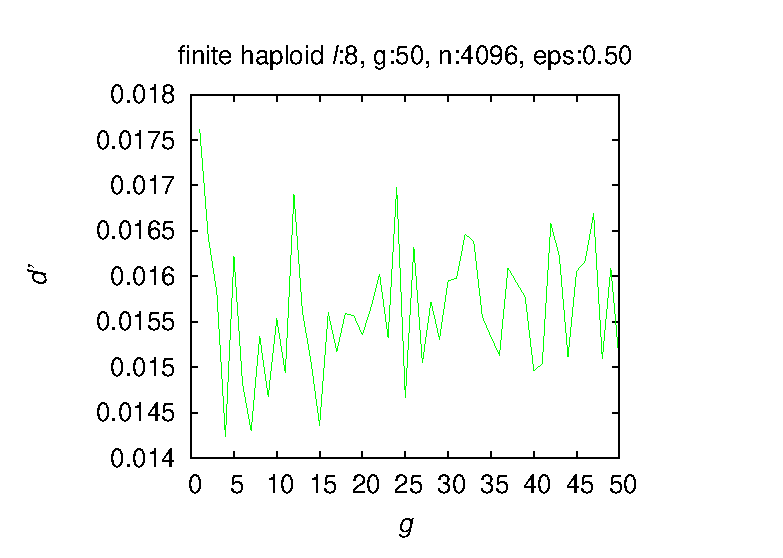
\includegraphics{figures/eps/vio/chi/b8/e0.5/n00004096_fin_hap.eps}}} \hspace{-3em}%
\subfloat{
\resizebox{8cm}{4.5cm}{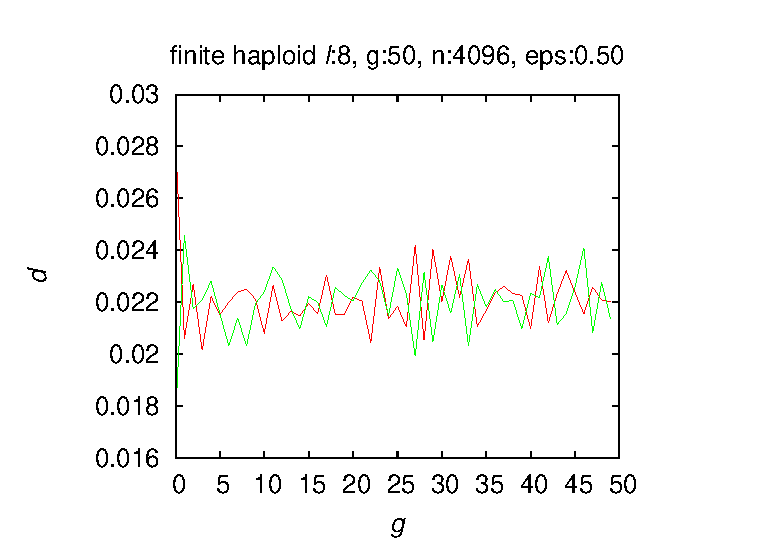
\includegraphics{figures/eps/vio/chi/b8/e0.5/n00004096_fin_hap_wovio.eps}}}\vspace{-1em} \hspace{-3em}%
\end{center}
\begin{center}
\subfloat{
\resizebox{8cm}{4.5cm}{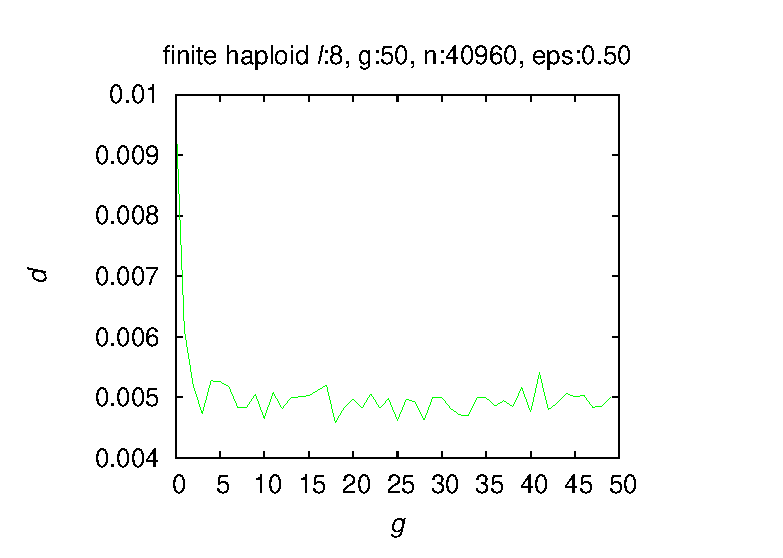
\includegraphics{figures/eps/vio/chi/b8/e0.5/n00040960_fin_hap.eps}}} \hspace{-3em}%
\subfloat{
\resizebox{8cm}{4.5cm}{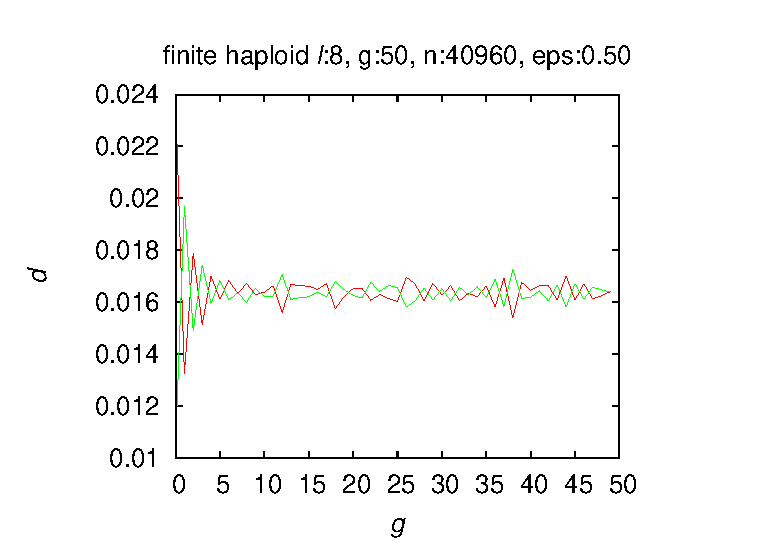
\includegraphics{figures/eps/vio/chi/b8/e0.5/n00040960_fin_hap_wovio.eps}}}\vspace{-1em} \hspace{-3em}%
\end{center}

\begin{center}
\subfloat{
\resizebox{8cm}{4.5cm}{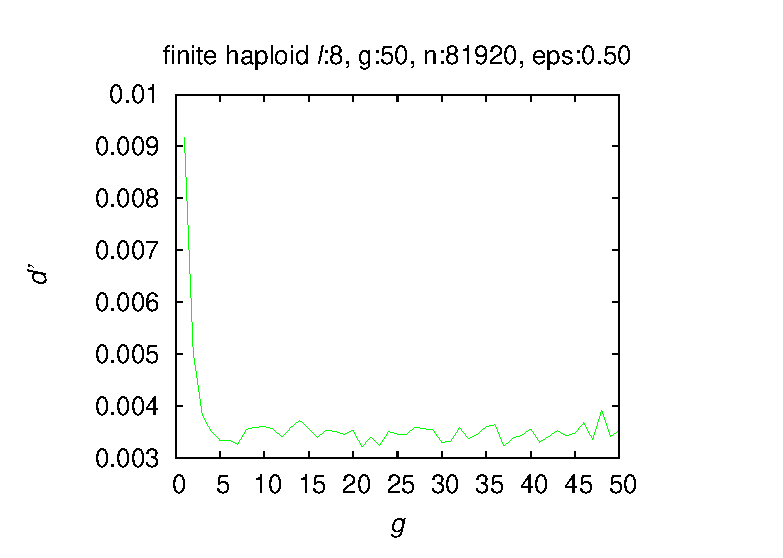
\includegraphics{figures/eps/vio/chi/b8/e0.5/n00081920_fin_hap.eps}}} \hspace{-3em}%
\subfloat{
\resizebox{8cm}{4.5cm}{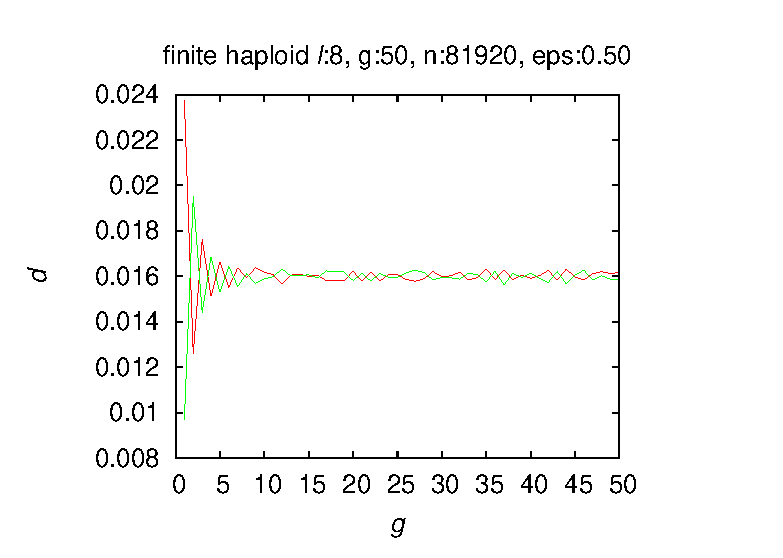
\includegraphics{figures/eps/vio/chi/b8/e0.5/n00081920_fin_hap_wovio.eps}}}\vspace{-1em} \hspace{-3em}%
\end{center}

\begin{center}
\subfloat{
\resizebox{8cm}{4.5cm}{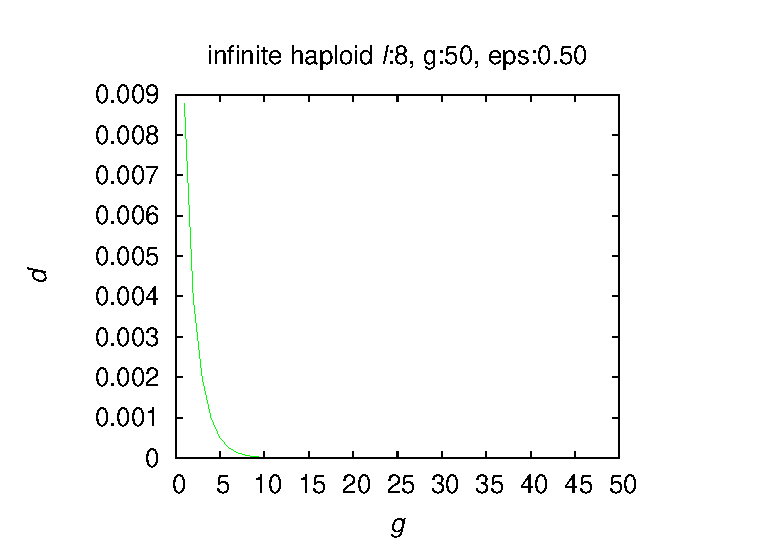
\includegraphics{figures/eps/vio/chi/b8/e0.5/inf_hap.eps}}}\hspace{-3em}%
\subfloat{
\resizebox{8cm}{4.5cm}{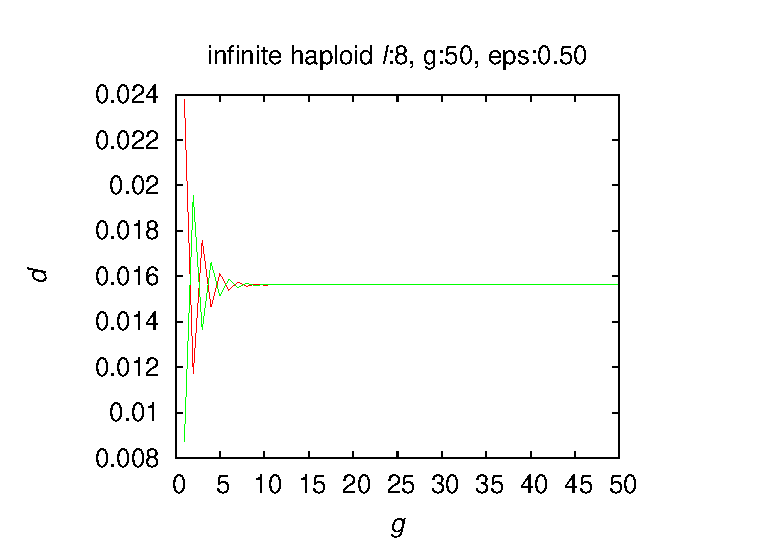
\includegraphics{figures/eps/vio/chi/b8/e0.5/inf_hap_wovio.eps}}}\vspace{-0.5em} \hspace{-3em}%


\caption[\textbf{Infinite and finite haploid population behavior for $\bm{\chi}$ violation, $\ell = 8$ and $\bm{\epsilon} = 0.5$}]
{\textbf{Infinite and finite haploid population behavior for $\bm{\chi}$ violation, $\ell = 8$ and $\bm{\epsilon} = 0.5$:} 
  In left column, $d'$ is distance of finite or infinite population to limit $\bm{z}^\ast$ for $g$ generations. 
  In right column, $d$ is distance of finite or infinite population to limits $\bm{p}^\ast$ and $\bm{q}^\ast$. Green line is distance to $\bm{p*}$ and red line is distance to $\bm{q*}$.}
\label{oscillation_8h_vio_chi_0.5}
\end{center}
\end{figure}


% l = 10

\begin{figure}[h]
\begin{center}
\subfloat{
\resizebox{8cm}{4.5cm}{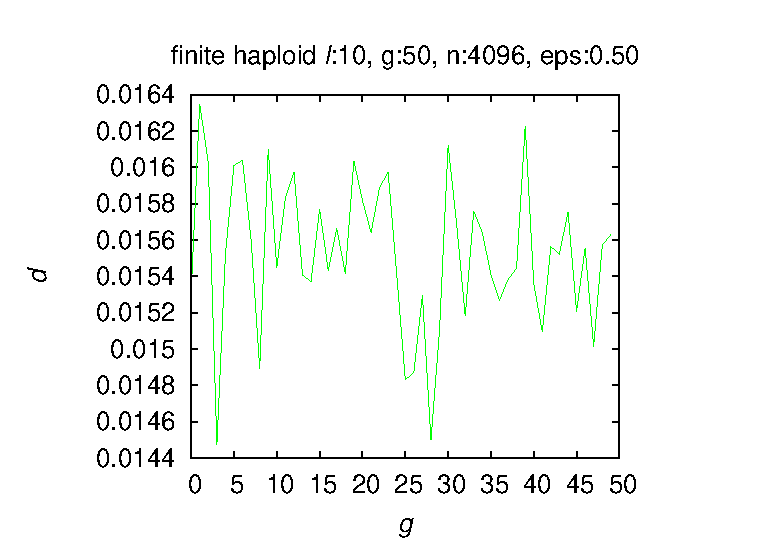
\includegraphics{figures/eps/vio/chi/b10/e0.5/n00004096_fin_hap.eps}}} \hspace{-3em}%
\subfloat{
\resizebox{8cm}{4.5cm}{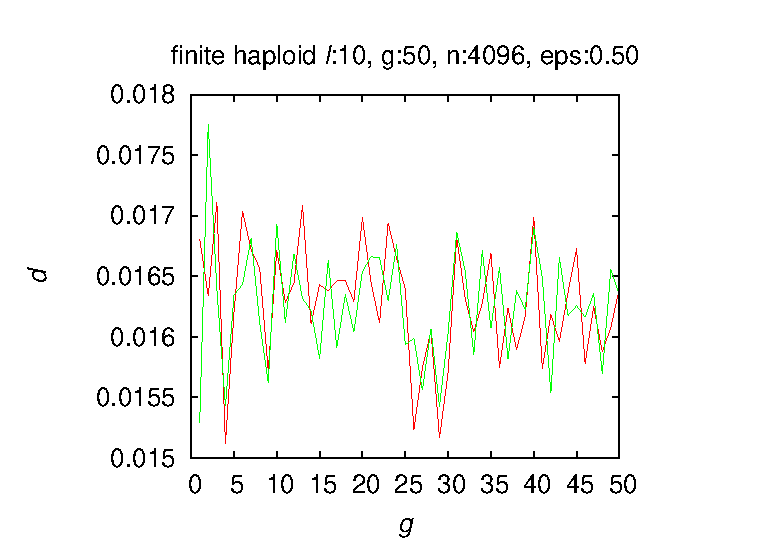
\includegraphics{figures/eps/vio/chi/b10/e0.5/n00004096_fin_hap_wovio.eps}}}\vspace{-1em} \hspace{-3em}%
\end{center}
\begin{center}
\subfloat{
\resizebox{8cm}{4.5cm}{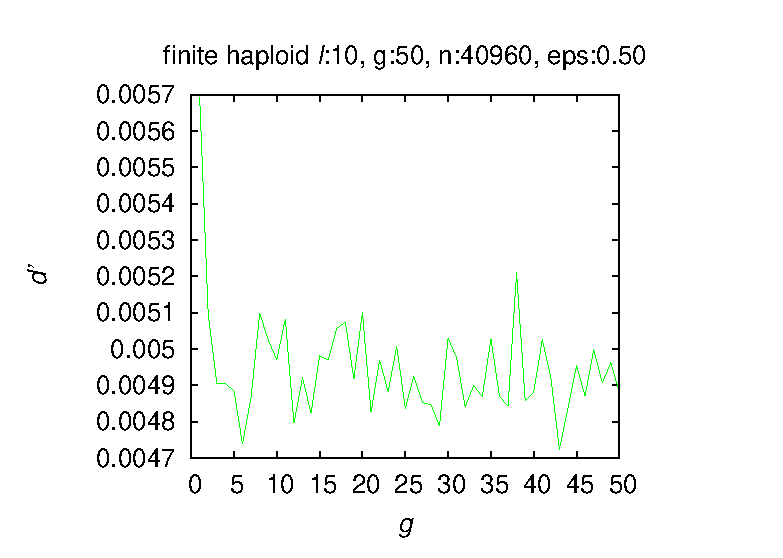
\includegraphics{figures/eps/vio/chi/b10/e0.5/n00040960_fin_hap.eps}}} \hspace{-3em}%
\subfloat{
\resizebox{8cm}{4.5cm}{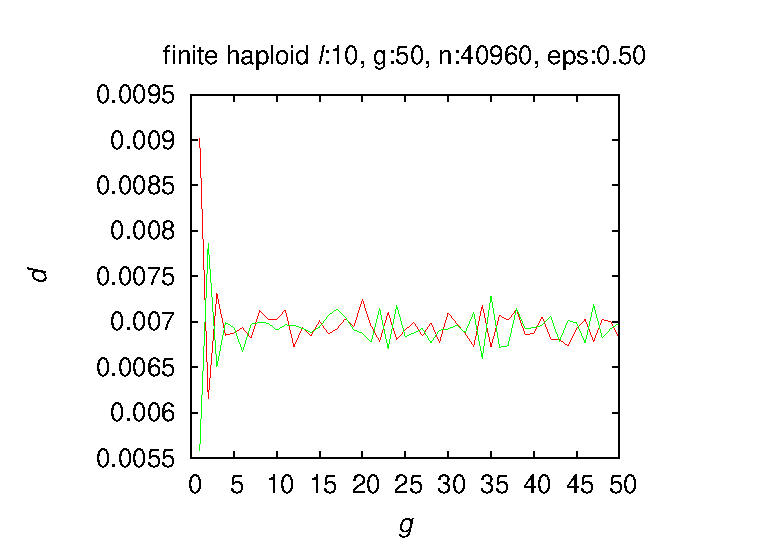
\includegraphics{figures/eps/vio/chi/b10/e0.5/n00040960_fin_hap_wovio.eps}}}\vspace{-1em} \hspace{-3em}%
\end{center}

\begin{center}
\subfloat{
\resizebox{8cm}{4.5cm}{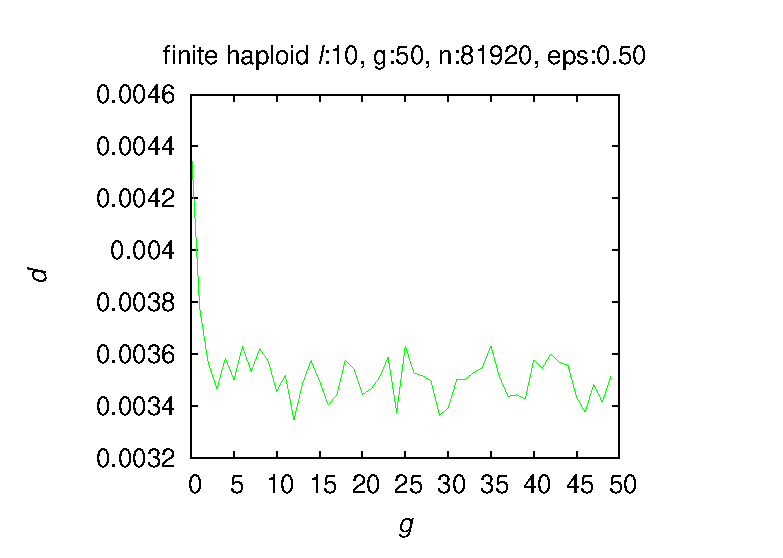
\includegraphics{figures/eps/vio/chi/b10/e0.5/n00081920_fin_hap.eps}}} \hspace{-3em}%
\subfloat{
\resizebox{8cm}{4.5cm}{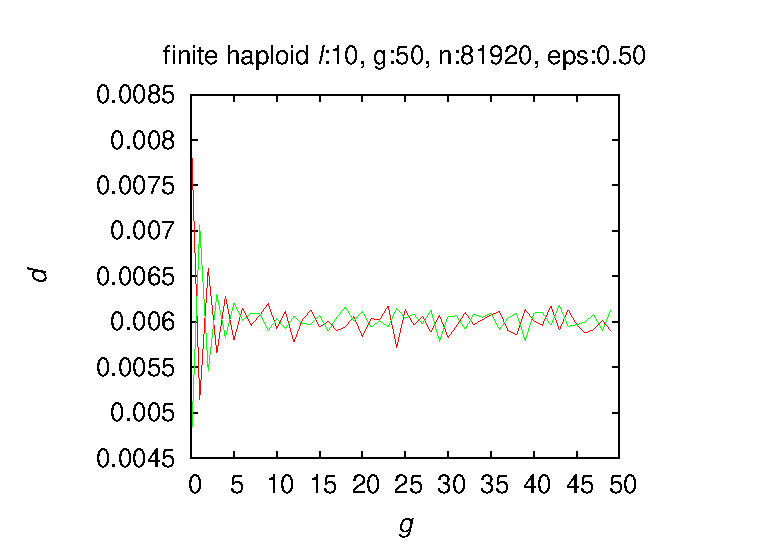
\includegraphics{figures/eps/vio/chi/b10/e0.5/n00081920_fin_hap_wovio.eps}}}\vspace{-1em} \hspace{-3em}%
\end{center}

\begin{center}
\subfloat{
\resizebox{8cm}{4.5cm}{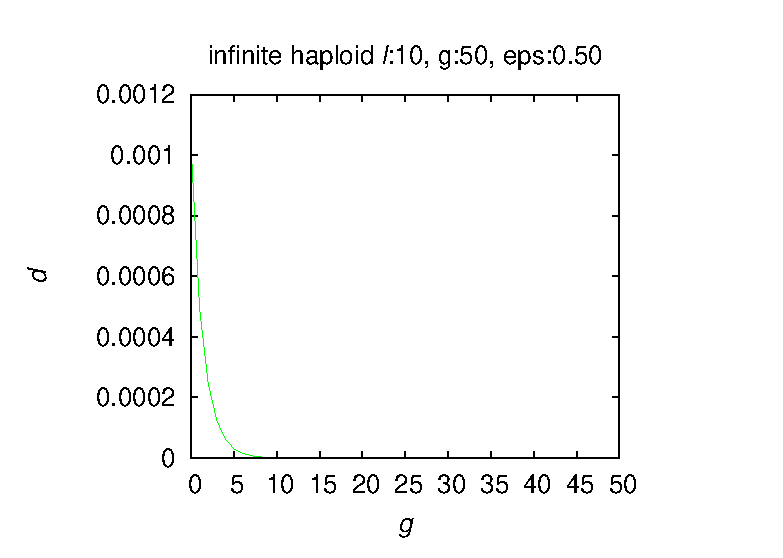
\includegraphics{figures/eps/vio/chi/b10/e0.5/inf_hap.eps}}}\hspace{-3em}%
\subfloat{
\resizebox{8cm}{4.5cm}{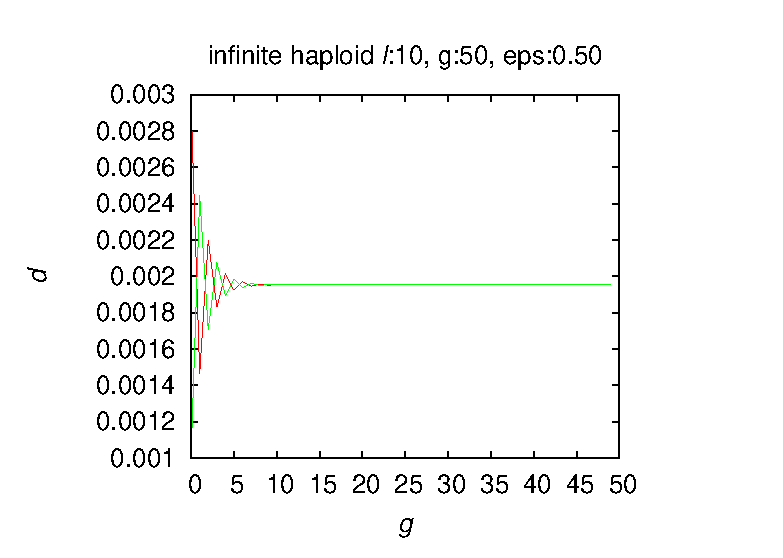
\includegraphics{figures/eps/vio/chi/b10/e0.5/inf_hap_wovio.eps}}}\vspace{-0.5em} \hspace{-3em}%

\caption[\textbf{Infinite and finite haploid population behavior for $\bm{\chi}$ violation, genome length $\ell = 10$ and $\bm{\epsilon} = 0.5$}]{\textbf{Infinite and finite haploid population behavior for $\bm{\chi}$ violation, genome length $\ell = 10$ and $\bm{\epsilon} = 0.5$:} 
  In left column, $d'$ is distance of finite or infinite population to limit $\bm{z}^\ast$ for $g$ generations. In right column, $d$ is distance of finite or infinite population to limits $\bm{p}^\ast$ and $\bm{q}^\ast$. Green line is distance to $\bm{p*}$ and red line is distance to $\bm{q*}$.}
\label{oscillation_10h_vio_chi_0.5}
\end{center}
\end{figure}

% l = 12
\begin{figure}[h]
\begin{center}
\subfloat{
\resizebox{8cm}{4.5cm}{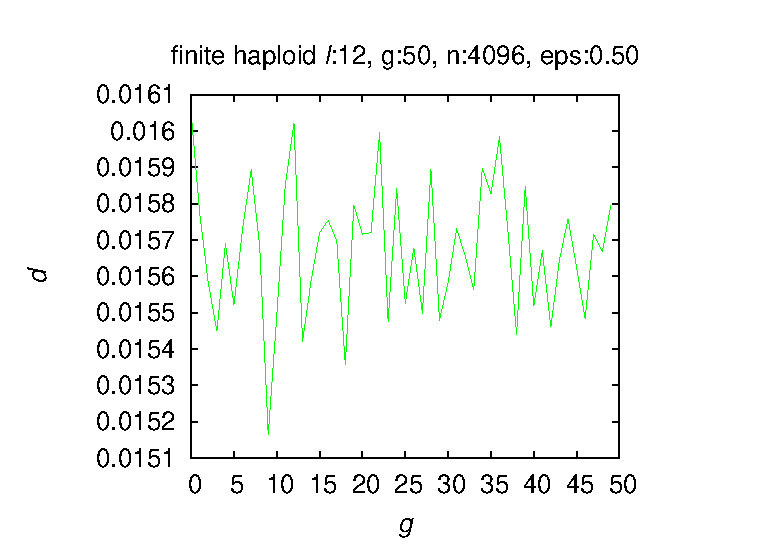
\includegraphics{figures/eps/vio/chi/b12/e0.5/n00004096_fin_hap.eps}}} \hspace{-3em}%
\subfloat{
\resizebox{8cm}{4.5cm}{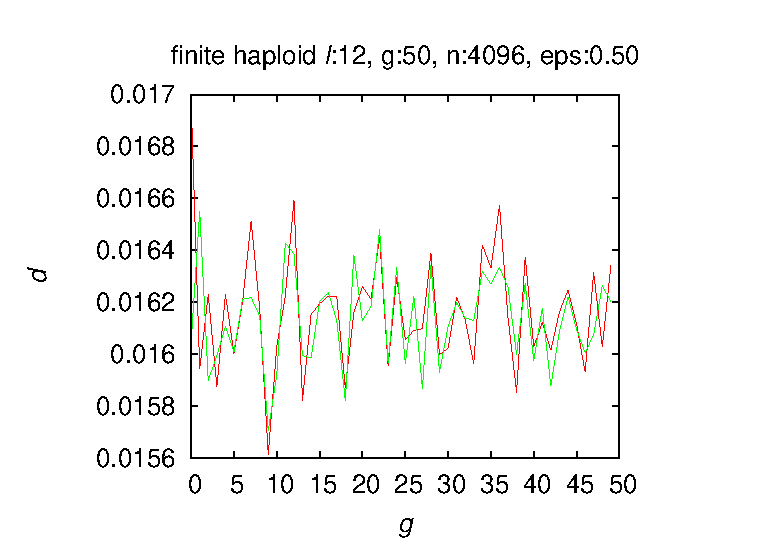
\includegraphics{figures/eps/vio/chi/b12/e0.5/n00004096_fin_hap_wovio.eps}}}\vspace{-1em} \hspace{-3em}%
\end{center}
\begin{center}
\subfloat{
\resizebox{8cm}{4.5cm}{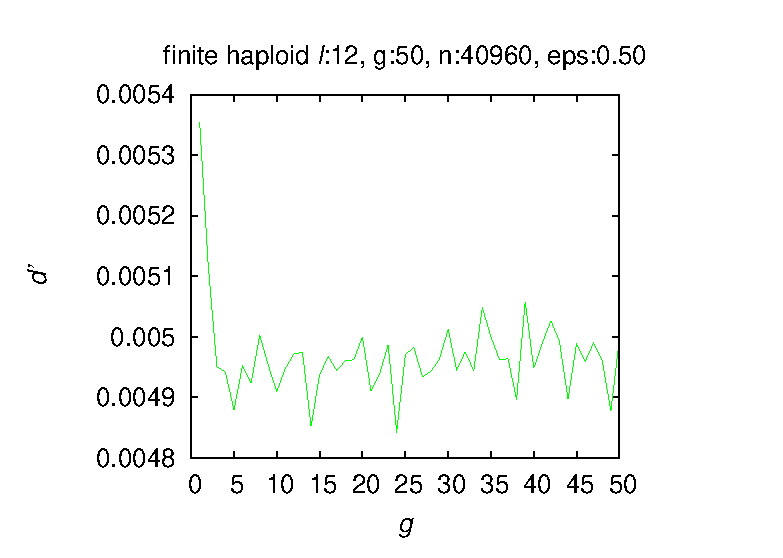
\includegraphics{figures/eps/vio/chi/b12/e0.5/n00040960_fin_hap.eps}}} \hspace{-3em}%
\subfloat{
\resizebox{8cm}{4.5cm}{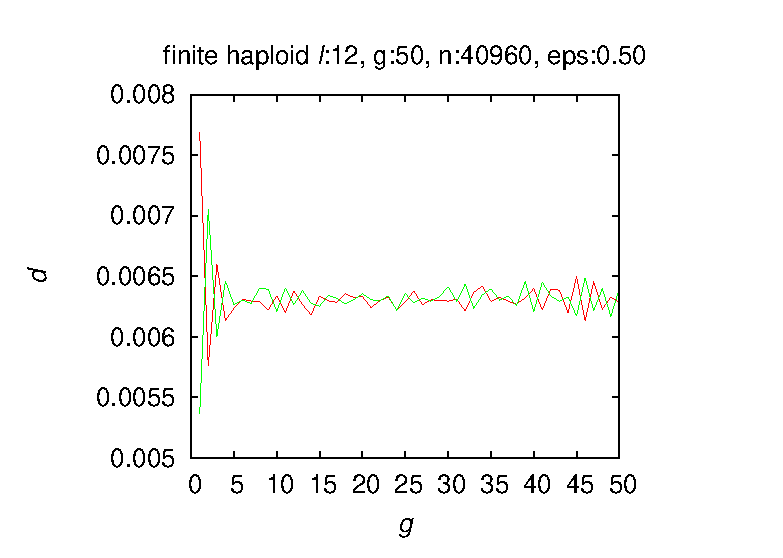
\includegraphics{figures/eps/vio/chi/b12/e0.5/n00040960_fin_hap_wovio.eps}}}\vspace{-1em} \hspace{-3em}%
\end{center}

\begin{center}
\subfloat{
\resizebox{8cm}{4.5cm}{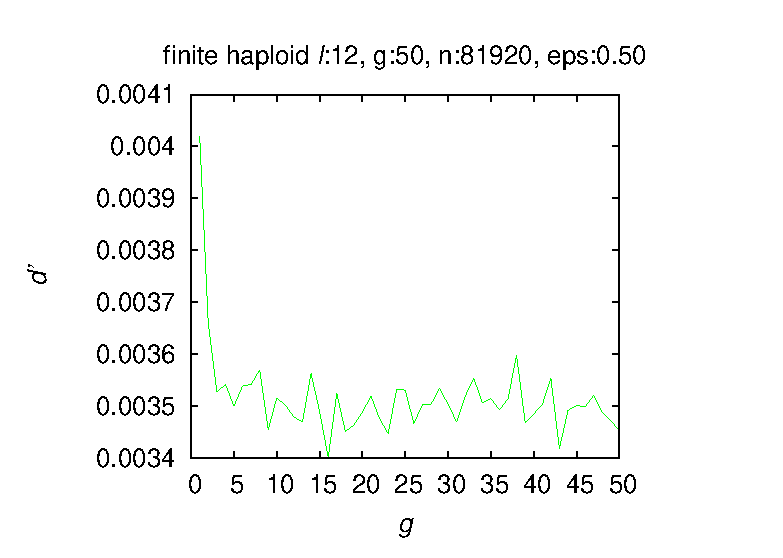
\includegraphics{figures/eps/vio/chi/b12/e0.5/n00081920_fin_hap.eps}}} \hspace{-3em}%
\subfloat{
\resizebox{8cm}{4.5cm}{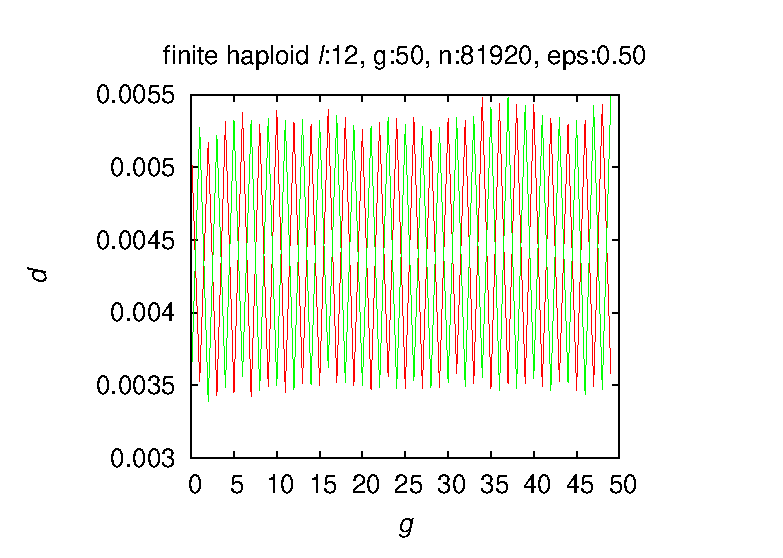
\includegraphics{figures/eps/vio/chi/b12/e0.5/n00081920_fin_hap_wovio.eps}}}\vspace{-1em} \hspace{-3em}%
\end{center}

\begin{center}
\subfloat{
\resizebox{8cm}{4.5cm}{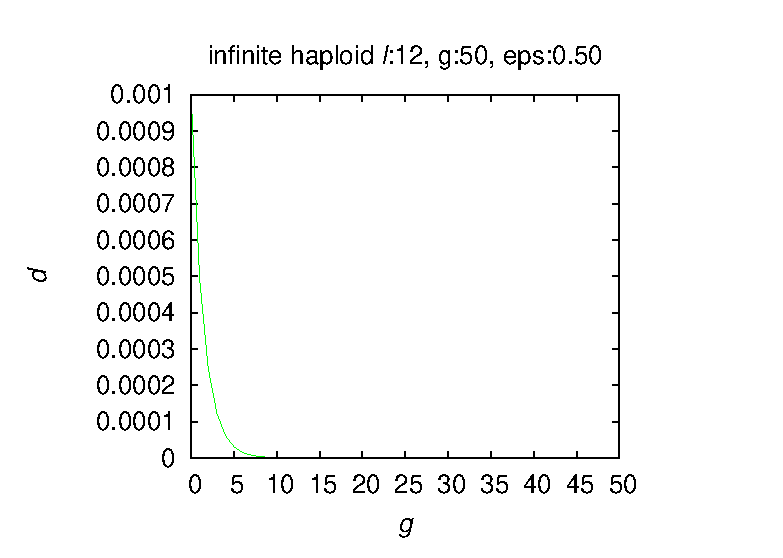
\includegraphics{figures/eps/vio/chi/b12/e0.5/inf_hap.eps}}}\hspace{-3em}%
\subfloat{
\resizebox{8cm}{4.5cm}{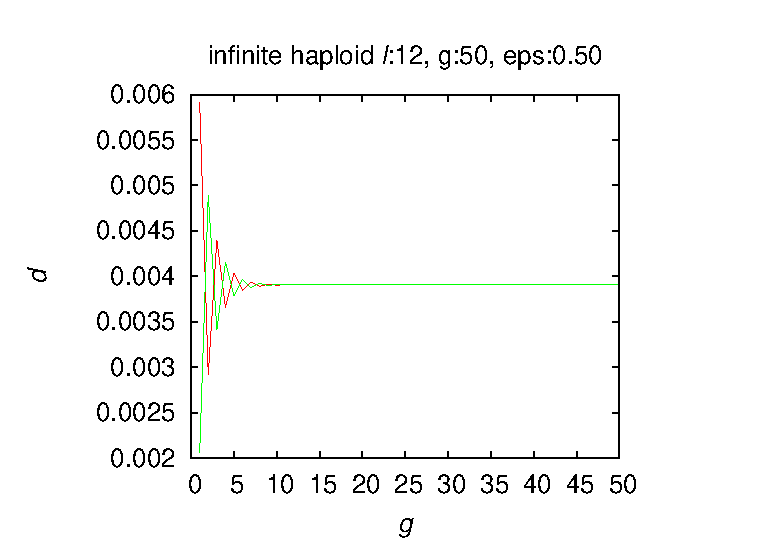
\includegraphics{figures/eps/vio/chi/b12/e0.5/inf_hap_wovio.eps}}}\vspace{-0.5em} \hspace{-3em}%


\caption[\textbf{Infinite and finite haploid population behavior for $\bm{\chi}$ violation, genome length $\ell = 12$ and $\bm{\epsilon} = 0.5$}]{\textbf{Infinite and finite haploid population behavior for $\bm{\chi}$ violation, genome length $\ell = 12$ and $\bm{\epsilon} = 0.5$:} 
  In left column, $d'$ is distance of finite or infinite population to limit $\bm{z}^\ast$ for $g$ generations. In right column, $d$ is distance of finite or infinite population to limits $\bm{p}^\ast$ and $\bm{q}^\ast$. Green line is distance to $\bm{p*}$ and red line is distance to $\bm{q*}$.}
\label{oscillation_12h_vio_chi_0.5}
\end{center}
\end{figure}

% l = 14

\begin{figure}[h]
\begin{center}
\subfloat{
\resizebox{8cm}{4.5cm}{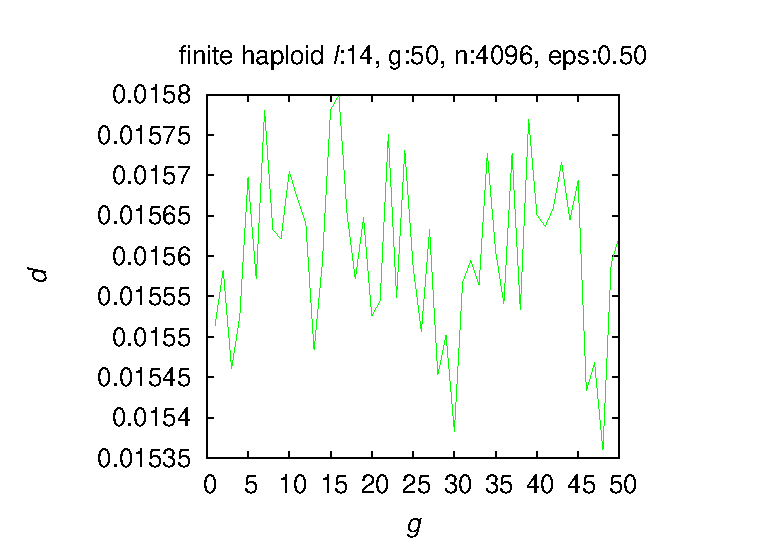
\includegraphics{figures/eps/vio/chi/b14/e0.5/n00004096_fin_hap.eps}}} \hspace{-3em}%
\subfloat{
\resizebox{8cm}{4.5cm}{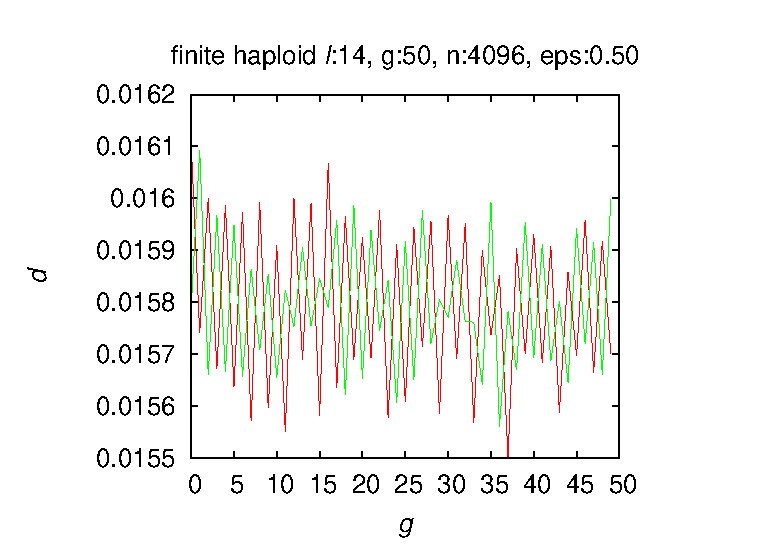
\includegraphics{figures/eps/vio/chi/b14/e0.5/n00004096_fin_hap_wovio.eps}}}\vspace{-1em} \hspace{-3em}%
\end{center}
\begin{center}
\subfloat{
\resizebox{8cm}{4.5cm}{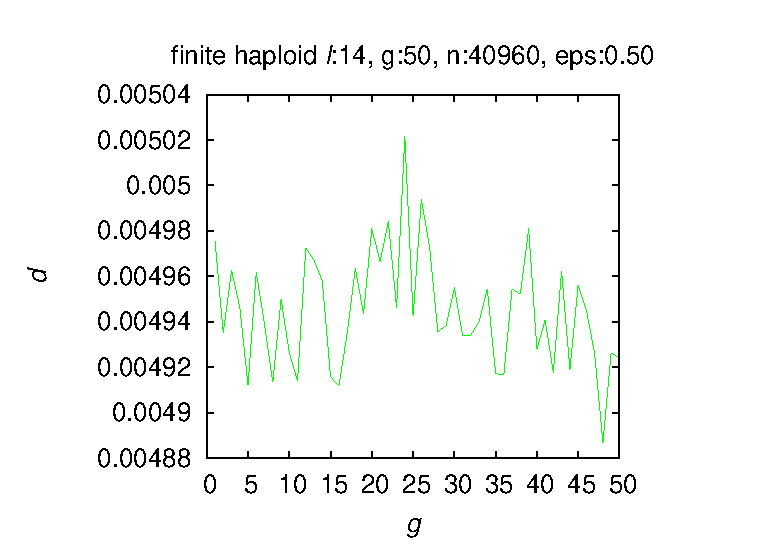
\includegraphics{figures/eps/vio/chi/b14/e0.5/n00040960_fin_hap.eps}}} \hspace{-3em}%
\subfloat{
\resizebox{8cm}{4.5cm}{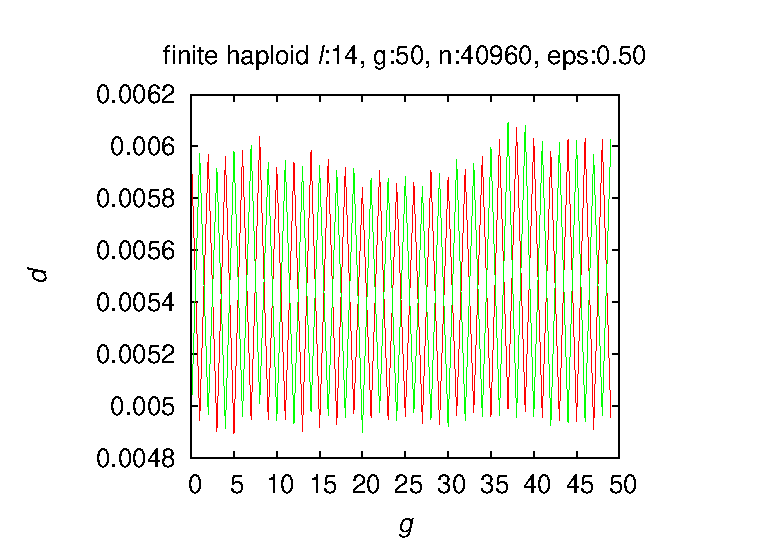
\includegraphics{figures/eps/vio/chi/b14/e0.5/n00040960_fin_hap_wovio.eps}}}\vspace{-1em} \hspace{-3em}%
\end{center}

\begin{center}
\subfloat{
\resizebox{8cm}{4.5cm}{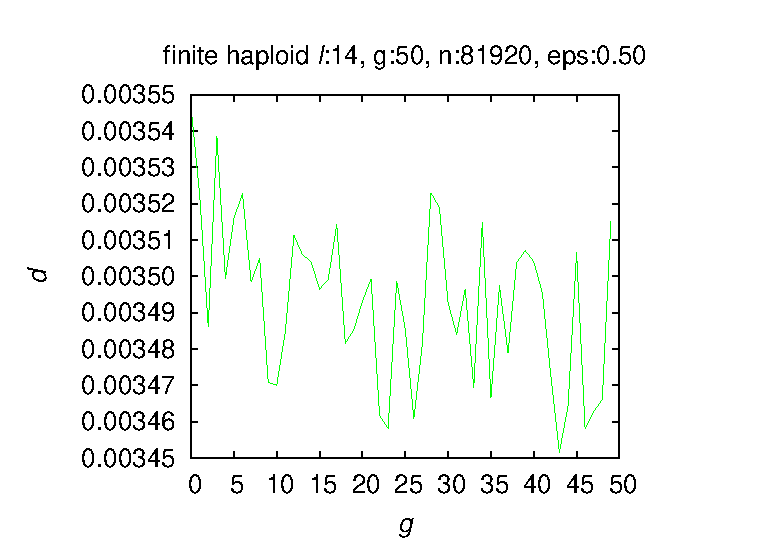
\includegraphics{figures/eps/vio/chi/b14/e0.5/n00081920_fin_hap.eps}}} \hspace{-3em}%
\subfloat{
\resizebox{8cm}{4.5cm}{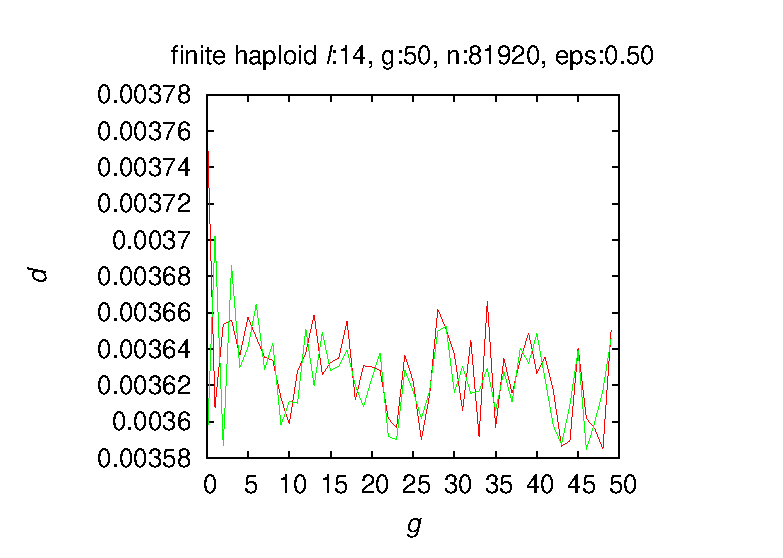
\includegraphics{figures/eps/vio/chi/b14/e0.5/n00081920_fin_hap_wovio.eps}}}\vspace{-1em} \hspace{-3em}%
\end{center}

\begin{center}
\subfloat{
\resizebox{8cm}{4.5cm}{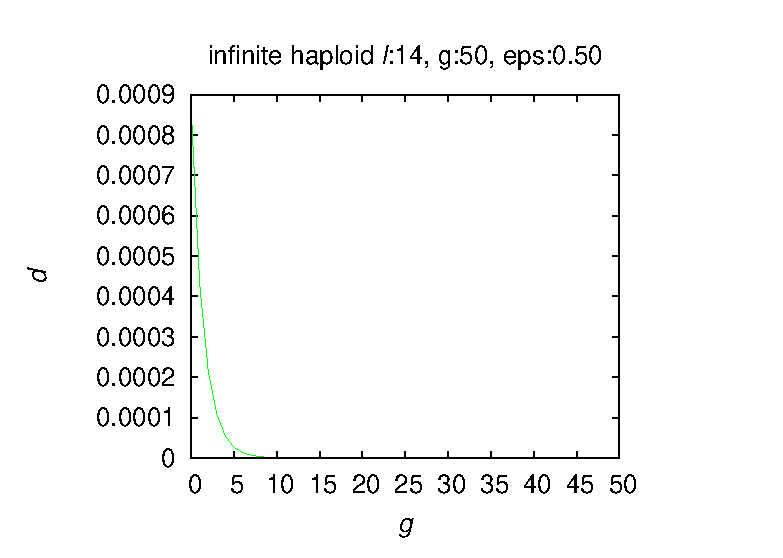
\includegraphics{figures/eps/vio/chi/b14/e0.5/inf_hap.eps}}}\hspace{-3em}%
\subfloat{
\resizebox{8cm}{4.5cm}{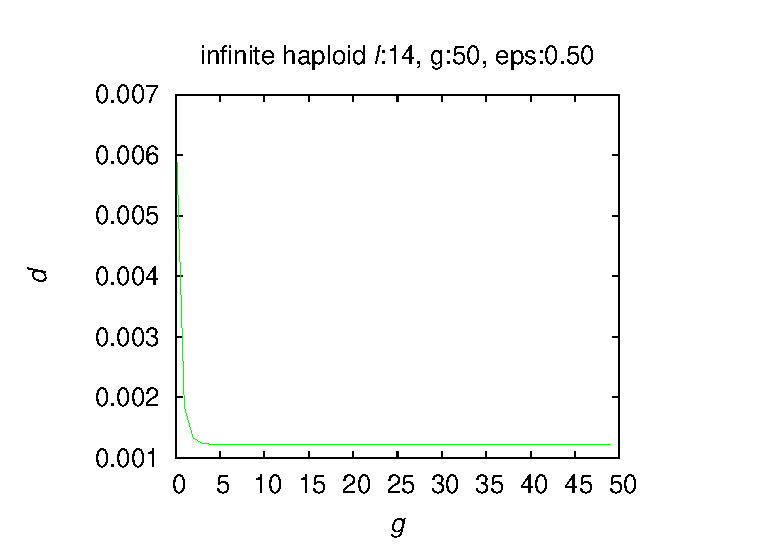
\includegraphics{figures/eps/vio/chi/b14/e0.5/inf_hap_wovio.eps}}}\vspace{-0.5em} \hspace{-3em}%

\caption[\textbf{Infinite and finite haploid population behavior for $\bm{\chi}$ violation, genome length $\ell = 14$ and $\bm{\epsilon} = 0.5$}]{\textbf{Infinite and finite haploid population behavior for $\bm{\chi}$ violation, genome length $\ell = 14$ and $\bm{\epsilon} = 0.5$:} 
  In left column, $d'$ is distance of finite or infinite population to limit $\bm{z}^\ast$ for $g$ generations. In right column, $d$ is distance of finite or infinite population to limits $\bm{p}^\ast$ and $\bm{q}^\ast$. Green line is distance to $\bm{p*}$ and red line is distance to $\bm{q*}$.}
\label{oscillation_14h_vio_chi_0.5}
\end{center}
\end{figure}

% \clearpage
The right column in figures \ref{oscillation_8h_vio_chi_0.5} through \ref{oscillation_14h_vio_chi_0.5} 
shows distance of finite and infinite haploid populations to non-violation limits $\bm{p^\ast}$ and $\bm{q^\ast}$ with $\bm{\epsilon} \;=\; 0.5$. 
The graphs indicate oscillating behavior. 
Unlike mutation with violation $\bm{\epsilon} \;=\; 0.5$, oscillation is observed for longer length of generations. 
Finite populations still show some though not very clear oscillations, and then show randomness in behavior as generation progresses. 
Infinite population also oscillates but the oscillation dies out quickly. Randomness in finite population behavior increases 
compared to smaller values of $\bm{\epsilon}$, especially as $\ell$ increases.

The left column of figures \ref{oscillation_8h_vio_chi_0.5} through \ref{oscillation_14h_vio_chi_0.5} 
shows distance of finite and infinite haploid populations to limit $\bm{z^\ast}$ 
(limit with violation in crossover distribution $\bm{\chi}$) when $\bm{\epsilon} \;=\; 0.5$. 
The distance decreases as population size increases, 
and finite population shows behavior similar to infinite population behavior as finite population size grows. 
Average distance data for haploid population in case of violation in $\bm{\chi}$ distribution 
with $\bm{\epsilon} \;=\; 0.5$ for different finite population size $N$ are tabulated in table \ref{distanceChiHapEps0.5}.

\clearpage
\begin{table}[h]
\caption[\textbf{Distance measured for violation in $\bm{\chi}$ with $\bm{\epsilon} \;=\; 0.5$  for haploids}]{\textbf{Distance measured for violation in $\bm{\chi}$ with $\bm{\epsilon} \;=\; 0.5$  for haploids:} $\ell$ is genome length, 
average distance between finite and infinite population is tabulated in the last three columns, and last row is expected single step distance.}
\centering
\begin{tabularx}{0.75\textwidth}{ c *{3}{X}}
\toprule
$\ell$ & $N = 4096$ & $N = 40960$ & $N = 81920$  \\
\midrule
8 & 0.0156	&  0.0051	& 0.0036 \\
10 & 0.0155	&  0.0049	& 0.0035 \\
12 & 0.0157	&  0.0050	& 0.0035 \\
14 & 0.0156	&  0.0049	& 0.0035 \\      
\midrule
$1/\sqrt{N}$ & 0.0156 & 0.0049 & 0.0035 \\
\bottomrule
\end{tabularx}
\label{distanceChiHapEps0.5}
\end{table} 

Table \ref{distanceChiHapEps0.5} shows that the average distance 
between finite and infinite populations approaches the expected single step distance $1/\sqrt{N}$. 








